\section{Clasificación supervisada: modelos grandes de lenguaje}
\label{sec:punto3}

% Punto 3 (10 puntos y 20 extra). Implementación: notebooks/tp2_detector_spam.ipynb. Pruebas: tests/test_punto3.py.

\subsection{Clasificación sin ajuste}

\paragraph{Modelo y prompt.} Para el punto 3.1 se usa
\texttt{Qwen/Qwen2.5-3B-Instruct}, un modelo decodificador de unos 3000
millones de parámetros ajustado para seguir instrucciones. Cada mensaje se
inserta \emph{sin preprocesar} en un prompt sin ejemplos, en inglés:
\begin{quote}\small\ttfamily
Classify the following SMS message as 'spam' or 'ham'. Answer with a single
word.\\[2pt]
Message: \{message\}\\
Answer:
\end{quote}
El prompt se envía como turno del usuario con la plantilla de chat del modelo.
No incluye ejemplos del dataset, de modo que ningún mensaje evaluado aparece
en las instrucciones.

\paragraph{Generación e interpretación.} La generación es voraz (sin
muestreo), con un máximo de 8 tokens nuevos, en GPU y con precisión de 16
bits. La respuesta se traduce a una etiqueta con la primera palabra
\texttt{spam} o \texttt{ham} que contiene; una negación como \emph{not spam}
cuenta como ham. Si la respuesta no contiene ninguna de las dos palabras, se
considera ham: así, un spam sin respuesta clara cuenta como spam no detectado.
Se informa cuántas respuestas fueron ambiguas.

\paragraph{Evaluación.} Con el modelo y la decodificación fijos, la
predicción de un mensaje no depende de la muestra en que aparece. Por eso cada
uno de los 5574 mensajes se clasifica una sola vez y las 30 muestras
estratificadas del 30\,\% (semillas 2026 a 2055) reutilizan esas predicciones.
El resultado es el mismo que clasificar cada muestra por separado. El modelo
no se entrena con el dataset, de modo que no hay fuga de entrenamiento hacia
las muestras. Sin embargo, las muestras se toman de todo el dataset y se
solapan entre sí, así que la variación entre corridas refleja solo el
muestreo. Los puntos 1 y 2 se evalúan, en cambio, sobre el 30\,\% de prueba
de cada partición.

\paragraph{Ejecución reproducible.} Se usó la revisión
\texttt{aa8e72537993ba99e69dfaafa59ed015b17504d1}, fijada tanto para el
tokenizador como para los pesos. La clasificación de los 5574 mensajes tardó
84.2 segundos en una NVIDIA GeForce RTX 3080 Ti de 12 GiB, bajo WSL2,
PyTorch \texttt{2.14.0+cu130}, precisión \texttt{bfloat16} y lotes de 16.
Este tiempo corresponde a la generación; excluye descarga y carga del modelo.
Los pesos ya estaban en caché. La generación se repitió con HF autenticado y
reprodujo exactamente las respuestas de la caché anterior. El token no forma
parte del notebook ni de los resultados. Después se liberó el modelo de la GPU.

\paragraph{Resultados.} En las 30 muestras, la tasa de aciertos fue
$0.7853\pm0.0073$ y el F1-score $0.5452\pm0.0090$ (media y desviación
estándar muestral). No hubo respuestas ambiguas. La tabla conserva los
resultados anteriores como referencia descriptiva: los protocolos de muestreo
son diferentes, por lo que no es una comparación pareada sobre las mismas filas.

\begin{table}[H]
\centering
\caption{Referencia de los puntos 1 y 2 frente a Qwen sin ajuste. Media y
desviación en 30 corridas; los LLM usan muestras del dataset completo.}
\begin{tabular}{lcc}
\toprule
Método & Tasa de aciertos & F1-score\\
\midrule
Regresión sin PCA & $0.9906\pm0.0016$ & $0.9641\pm0.0063$\\
Histogramas, $D=2$ & $0.9195\pm0.0084$ & $0.7043\pm0.0247$\\
Qwen2.5-3B-Instruct & $0.7853\pm0.0073$ & $0.5452\pm0.0090$\\
\bottomrule
\end{tabular}
\end{table}

\begin{figure}[H]
\centering
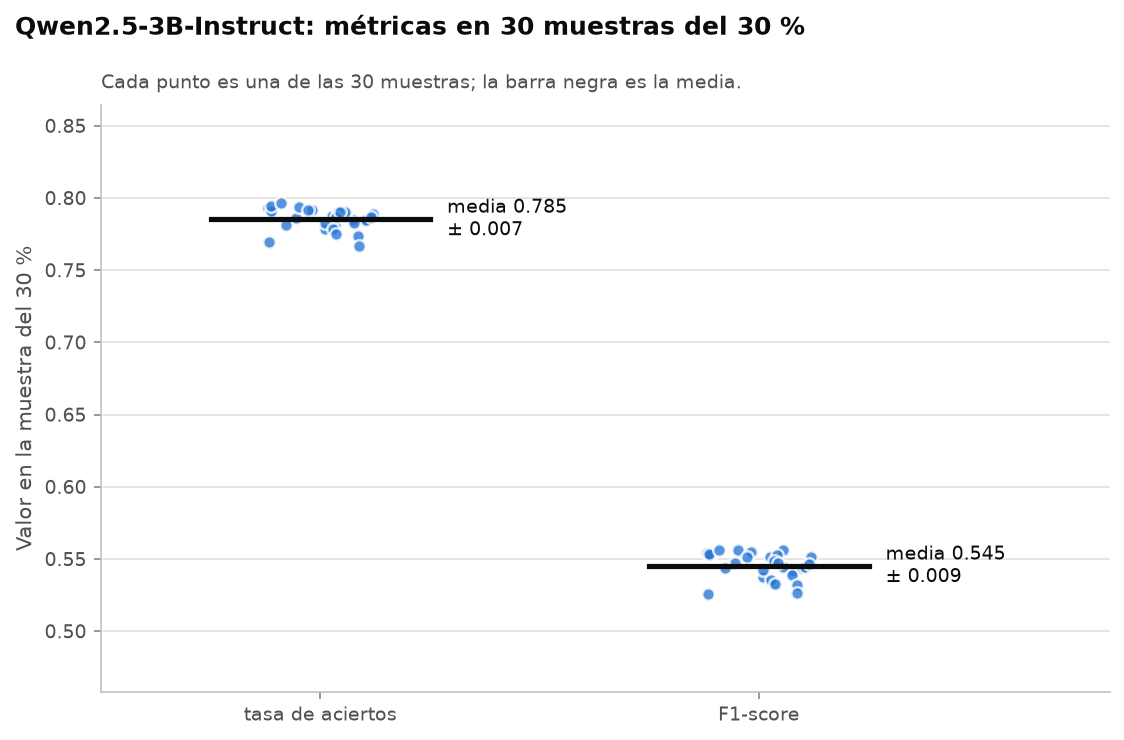
\includegraphics[width=\linewidth]{qwen2-5-3b-instruct-metricas-en-30-muestras-del-30.png}
\caption{Variación entre muestras de las predicciones fijas de Qwen; no
representa variación entre entrenamientos del modelo.}
\end{figure}

\paragraph{Errores y alcance.} Sobre todo el dataset, Qwen detectó 717 de
747 spam (recobrado 96.0\,\%), pero marcó como spam 1168 de los 4827 ham
(24.2\,\%). La precisión de spam fue 38.0\,\%: predijo 1885 spam, de los
cuales solo 717 eran correctos. En las muestras hubo, en promedio, 349.9
falsos positivos y 9.0 falsos negativos. El F1 bajo se explica principalmente
por las falsas alarmas, no por respuestas ambiguas. Incluso la tasa de
aciertos queda por debajo de predecir siempre ham (86.6\,\% en el dataset),
aunque esa regla trivial tendría F1 cero para spam.

\begin{figure}[H]
\centering
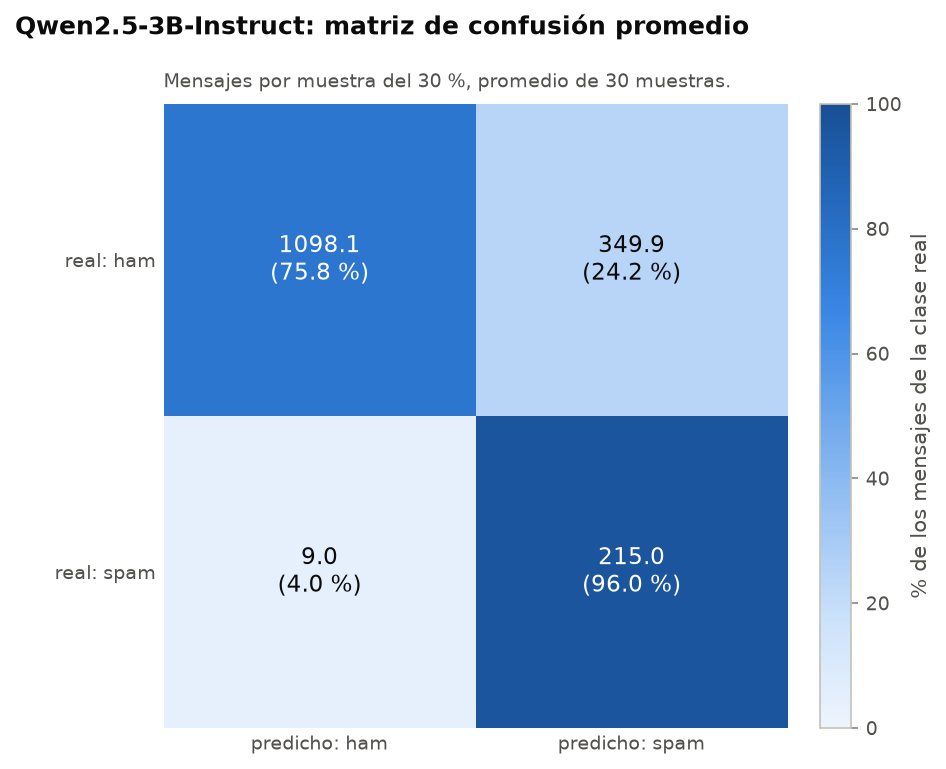
\includegraphics[width=0.86\linewidth]{qwen2-5-3b-instruct-matriz-de-confusion-promedio.png}
\caption{Confusión promedio de Qwen. La abundancia de ham marcado como spam
limita la precisión a pesar de detectar la mayor parte del spam.}
\end{figure}

Este resultado corresponde al modelo, prompt sin ejemplos y decodificación
confirmados. No se cambió el prompt después de observar las métricas.
Tampoco permite concluir que cualquier LLM sea inferior: evalúa esta
configuración concreta. Quedan pendientes los dos modelos adicionales de
3.2, si el equipo decide realizar el extra.

\subsection{Ajuste fino eficiente}

TODO (punto 3.3, extra): describir el ajuste con LoRA \cite{hu2021lora} o
DoRA \cite{liu2024dora} y analizar sus resultados.
